\chapter{कार्बोक्सिलिक अम्ल व्युत्पन्न}\label{ch:b2:acyl-substitution}

जैतून के तेल को सोडियम हाइड्रॉक्साइड के साथ उबालिए और आपको साबुन और ग्लिसरॉल मिलते हैं: यह
जान-बूझकर चलाई गई सबसे पुरानी कार्बनिक अभिक्रिया है। तेल ग्लिसरॉल और
लंबी शृंखला वाले अम्लों का एस्टर है, और हाइड्रॉक्साइड हर एस्टर को एक आबंध पर काटता है, सदैव
उसी आबंध पर, कार्बोनिल कार्बन और ऐल्कोहॉल के ऑक्सीजन के बीच। एस्टर,
अम्ल, ऐमाइड, ऐनहाइड्राइड और \omterm{def:b2:acyl-substitution:derivative}{ऐसिल क्लोराइड} सभी इसी प्रकार अभिक्रिया करते हैं: एक
नाभिकरागी कार्बोनिल कार्बन से जुड़ता है, और एक समूह निकल जाता है। इन यौगिकों को
इस आधार पर क्रमबद्ध करना कि उनका समूह कितनी अच्छी तरह निकलता है, बताता है कि किसे किसमें बदला जा सकता है,
और किस दिशा में किसी रसायनज्ञ को चढ़ाई करनी पड़ती है।

\begin{recall}
प्रथम वर्ष का खंड: कार्बोनिल समूह का इलेक्ट्रॉनरागी सक्रियण, हेमीऐसीटैल और
ऐसीटैल बनने की क्रियाविधियाँ, कार्बमैग्नीशियम योग, हाइड्राइड दाता और उनका कार्यक्षेत्र, निर्गामी समूह,
$\mathrm pK_a$, $Q$ और $K$। \Cref{ch:b2:amines}: \omterm{def:b2:amines:nucleophilic-addition}{नाभिकरागी योग}, ऐमीन।
\Cref{ch:b2:equilibrium-shifts}: \omterm{def:b2:equilibrium-shifts:shift}{साम्य का विस्थापन}। विद्यालय का खंड: एस्टर, कार्बोक्सिलिक अम्ल
और ऐमाइड।
\end{recall}

\begin{omfigure}
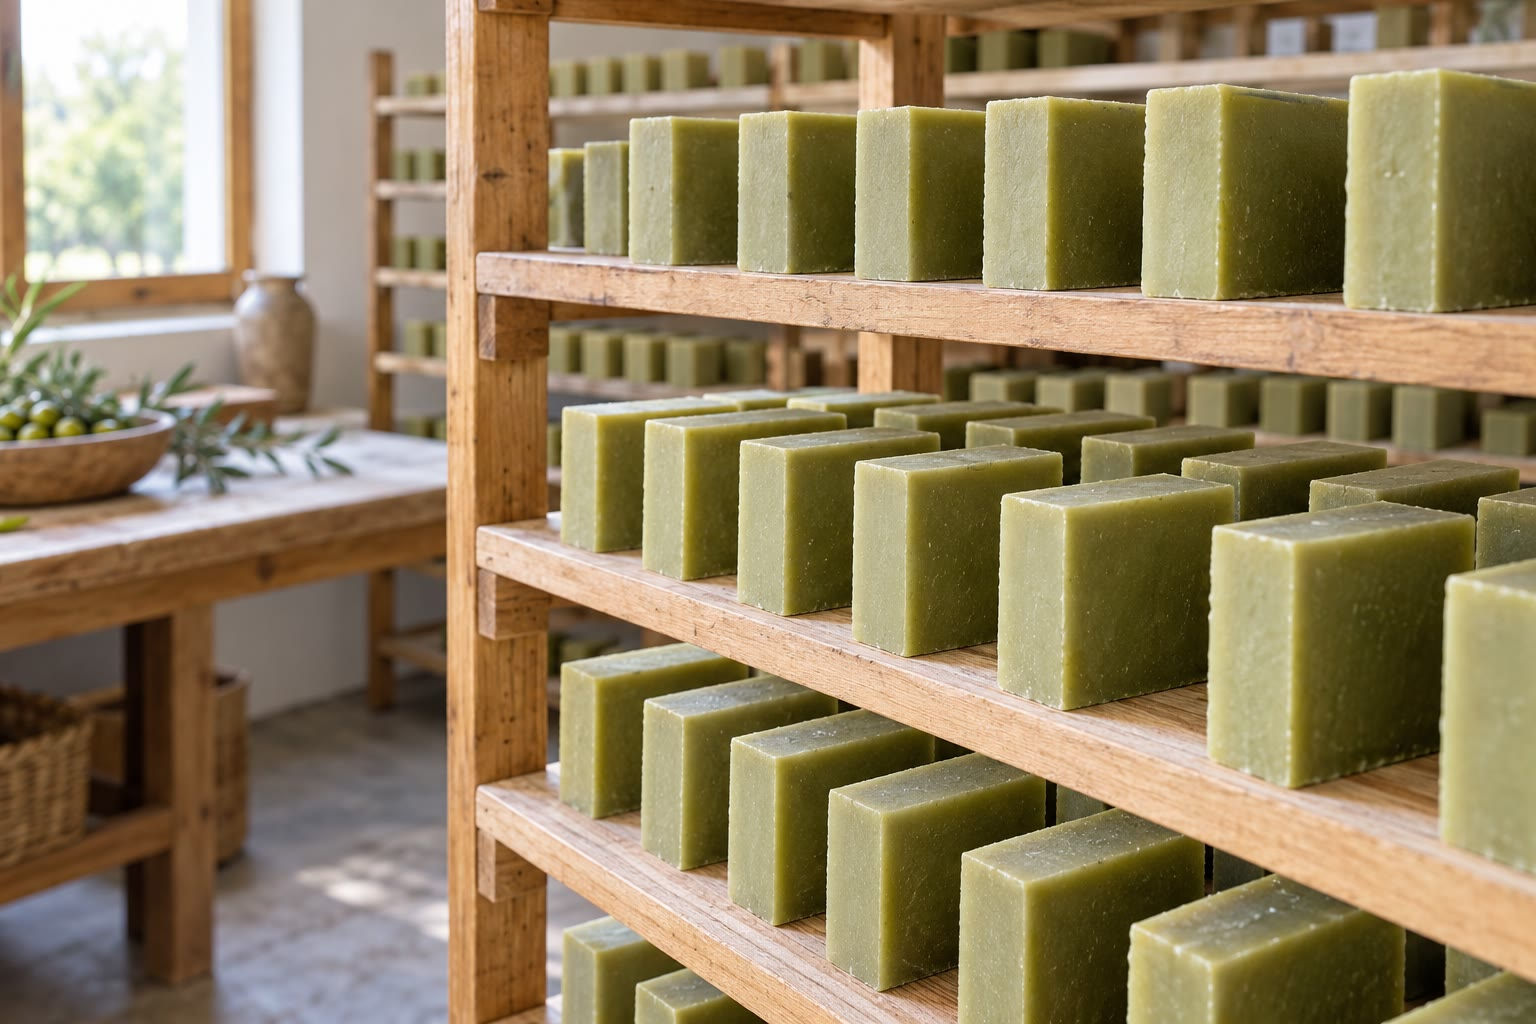
\includegraphics[width=0.58\linewidth]{images/book3/ai/b2-24-soap-bars.jpg}

{\small लकड़ी के रैकों पर सूखती जैतून-तेल साबुन की टिकियाँ। साबुन उन वसा अम्लों का सोडियम लवण है
जो तेल, एक एस्टर, को सोडियम हाइड्रॉक्साइड के साथ उबालने पर मुक्त होते हैं।}
\end{omfigure}

\section{परिवार और उसकी अभिक्रियाशीलता}

\begin{definition}[कार्बोक्सिलिक अम्ल व्युत्पन्न]\label{def:b2:acyl-substitution:derivative}
\emph{कार्बोक्सिलिक अम्ल व्युत्पन्न}\index{कार्बोक्सिलिक अम्ल व्युत्पन्न} एक यौगिक \ce{R-CO-Z} है जिसमें
किसी कार्बोक्सिलिक अम्ल का \ce{OH} किसी अन्य समूह Z से प्रतिस्थापित हो। \emph{ऐसिल
समूह}\index{ऐसिल समूह} $\mathrm{R{-}CO{-}}$ इन सभी में उभयनिष्ठ है। \emph{ऐसिल क्लोराइड}\index{ऐसिल क्लोराइड} में
Z, Cl है; \emph{अम्ल ऐनहाइड्राइड}\index{अम्ल ऐनहाइड्राइड} में Z, $\mathrm{O{-}CO{-}R'}$ है, अर्थात् एक ऑक्सीजन साझा करने वाले दो ऐसिल
समूह; एस्टर में Z, $\mathrm{OR'}$ है, ऐमाइड में $\mathrm{NR'_2}$।
\end{definition}

\begin{proposition}[अभिक्रियाशीलता पैमाना]\label{prop:b2:acyl-substitution:reactivity}
नाभिकरागियों के प्रति व्युत्पन्न इस क्रम में अभिक्रिया करते हैं: \omterm{def:b2:acyl-substitution:derivative}{ऐसिल क्लोराइड} $>$ ऐनहाइड्राइड $>$ एस्टर
$\approx$ अम्ल $>$ ऐमाइड।
\end{proposition}

\begin{proof}[तर्क]
दो प्रभाव जुड़ते हैं। निर्गामी समूह \ce{Z-} उतनी ही आसानी से निकलता है जितना दुर्बल क्षारक वह है:
\ce{Cl-} (संयुग्मी अम्ल \ce{HCl}, $\mathrm pK_a$ लगभग $-7$) किसी कार्बोक्सिलेट
($\mathrm pK_a$ लगभग 5), किसी ऐल्कॉक्साइड (लगभग 16) या किसी ऐमाइड आयन (लगभग 35) से कहीं बेहतर। और समूह Z
अपने एकाकी युग्म के मेसोमेरी दान द्वारा कार्बोनिल को इलेक्ट्रॉन घनत्व देता है, जो कार्बोनिल
कार्बन को कम इलेक्ट्रॉनरागी बनाता है: Cl के लिए दुर्बल, नाइट्रोजन के लिए सबसे प्रबल। ऐमाइड सबसे क्षीण
इलेक्ट्रॉनरागी भी है और सबसे क्षीण निर्गामी समूह भी।
% ledger: pka:ethanoic, pka:ethanol
\end{proof}

\section{नाभिकरागी ऐसिल प्रतिस्थापन}

\begin{definition}[नाभिकरागी ऐसिल प्रतिस्थापन]\label{def:b2:acyl-substitution:nas}
\emph{नाभिकरागी ऐसिल प्रतिस्थापन}\index{नाभिकरागी ऐसिल प्रतिस्थापन} किसी ऐसिल यौगिक के समूह Z
को किसी नाभिकरागी से प्रतिस्थापित करता है। यह कार्बोनिल कार्बन पर नाभिकरागी के योग से आगे बढ़ता है,
जो एक \emph{चतुष्फलकीय मध्यवर्ती}\index{चतुष्फलकीय मध्यवर्ती} देता है, और उसके बाद
निर्गामी समूह के विलोपन से, जो \ce{C=O} आबंध को पुनः स्थापित करता है।
\end{definition}

\begin{proposition}[योग--विलोपन]\label{prop:b2:acyl-substitution:addition-elimination}
ऐसिल प्रतिस्थापन एक \omterm{def:b2:acyl-substitution:nas}{चतुष्फलकीय मध्यवर्ती} से होकर जाता है; क्षारक में यह प्रबलतर
नाभिकरागी द्वारा और अम्ल में कार्बोनिल के सक्रियण द्वारा त्वरित होता है।
\end{proposition}

\begin{proof}[तर्क]
समतलीय और इलेक्ट्रॉनरागी कार्बोनिल कार्बन नाभिकरागी को अपने तल के ऊपर या नीचे से
ग्रहण करता है, जैसे \cref{ch:b2:amines} के योगों में; निकल सकने वाले समूह Z के साथ मध्यवर्ती
प्रोटॉनित होने के बजाय उसे बाहर निकाल देता है। क्षारक में नाभिकरागी एक ऋणायन है (\ce{HO-},
\ce{RO-}); अम्ल में कार्बोनिल ऑक्सीजन प्रोटॉनित होता है और कोई उदासीन नाभिकरागी (जल, कोई ऐल्कोहॉल)
पर्याप्त होता है। ऐल्कोहॉल भाग में \ce{^{18}O} से चिह्नित एस्टर जल-अपघटन पर चिह्नित ऐल्कोहॉल
और अचिह्नित अम्ल देते हैं: टूटने वाला आबंध ऐसिल--ऑक्सीजन आबंध है, जैसा क्रियाविधि माँगती है।
\end{proof}

\begin{omfigure}
\setchemfig{atom sep=1.7em}
\schemestart
\chemfig{R-C(=[2]O)-OR'} \+ \chemfig{HO^{-}}
\arrow{->[योग]}
\chemfig{R-C(-[2]O^{-})(-[6]OH)-OR'}
\arrow{->[विलोपन]}[,1.3]
\chemfig{R-C(=[2]O)-OH} \+ \chemfig{^{-}OR'}
\schemestop

\medskip
\schemestart
\chemfig{R-C(=[2]O)-OH} \+ \chemfig{^{-}OR'}
\arrow{->[प्रोटॉन स्थानांतरण]}
\chemfig{R-C(=[2]O)-O^{-}} \+ \chemfig{HOR'}
\schemestop
\par\vspace{6pt}

{\small किसी एस्टर का \omterm{def:b2:acyl-substitution:saponification}{साबुनीकरण}। हाइड्रॉक्साइड कार्बोनिल कार्बन से जुड़ता है, जिससे \omterm{def:b2:acyl-substitution:nas}{चतुष्फलकीय
मध्यवर्ती} बनता है; ऐल्कॉक्साइड निकलता है और \ce{C=O} आबंध फिर बनता है; फिर ऐल्कॉक्साइड, एक प्रबल क्षारक,
अम्ल का प्रोटॉन ले लेता है। यही अंतिम चरण अभिक्रिया को पूर्ण बनाता है।}
\end{omfigure}

\begin{method}[ऐसिल प्रतिस्थापन खींचना]\label{met:b2:acyl-substitution:nas-mechanism}
\begin{enumerate}
  \item क्षारक में: ऋणायनी नाभिकरागी कार्बोनिल कार्बन से जुड़ता है; ऋणात्मक आवेश
        ऑक्सीजन पर जाता है; \ce{C=O} आबंध फिर बनता है और Z निकलता है; अंत में कोई अम्ल--क्षारक चरण हो तो उसे लिखिए।
  \item अम्ल में: कार्बोनिल ऑक्सीजन को प्रोटॉनित कीजिए; उदासीन नाभिकरागी जुड़ता है; एक प्रोटॉन
        निर्गामी समूह पर स्थानांतरित कीजिए; वह उदासीन अणु के रूप में निकलता है; कार्बोनिल को विप्रोटॉनित कीजिए।
  \item चरण गिनिए: हर मध्यवर्ती या तो चतुष्फलकीय है या कोई कार्बोनिल यौगिक।
\end{enumerate}
\end{method}

\section{एस्टर}

\begin{definition}[एस्टरीकरण]\label{def:b2:acyl-substitution:esterification}
\emph{एस्टरीकरण}\index{एस्टरीकरण} किसी कार्बोक्सिलिक अम्ल (या किसी अधिक
अभिक्रियाशील व्युत्पन्न) और किसी ऐल्कोहॉल से एस्टर बनाता है। किसी प्रबल अम्ल द्वारा उत्प्रेरित,
अम्ल और ऐल्कोहॉल की प्रत्यक्ष अभिक्रिया फ़िशर एस्टरीकरण है।
\end{definition}

\begin{proposition}[फ़िशर एस्टरीकरण]\label{prop:b2:acyl-substitution:fischer}
फ़िशर \omterm{def:b2:acyl-substitution:esterification}{एस्टरीकरण} एक धीमा साम्य है, जिसका स्थिरांक प्राथमिक ऐल्कोहॉलों के लिए 4 के निकट है; इसे
किसी एक अभिकर्मक के आधिक्य से या बनते ही जल को हटाकर आगे बढ़ाया जाता है।
\end{proposition}

\begin{proof}[तर्क]\emergencystretch=3em
समान मोल एथेनॉल और एथेनोइक अम्ल तब रुकते हैं जब दो-तिहाई अम्ल एस्टरीकृत हो जाता है: $K =
(2/3)^2/(1/3)^2 = 4$। ऐल्कोहॉल के आधिक्य से, या जल को आसवित करके हटाने से
(प्रथम वर्ष के खंड का डीन--स्टार्क पात्र), $Q < K$ बनाए रखने पर अभिक्रिया और आगे बढ़ती है
(\cref{ch:b2:equilibrium-shifts})। क्रियाविधि के छह चरण अम्ल में \cref{met:b2:acyl-substitution:nas-mechanism}
के चरण हैं, सभी उत्क्रमणीय।
% ledger: ester:berthelot
\end{proof}

\begin{definition}[साबुनीकरण]\label{def:b2:acyl-substitution:saponification}
\emph{साबुनीकरण}\index{साबुनीकरण} किसी हाइड्रॉक्साइड द्वारा एस्टर का जल-अपघटन है, जो
कार्बोक्सिलेट लवण और ऐल्कोहॉल देता है।
\end{definition}

\begin{proposition}[साबुनीकरण पूर्ण होता है]\label{prop:b2:acyl-substitution:saponification}
\omterm{def:b2:acyl-substitution:saponification}{साबुनीकरण} पूर्णता तक जाता है: उसके अंतिम चरण, कार्बोक्सिलिक अम्ल से
ऐल्कॉक्साइड पर प्रोटॉन स्थानांतरण, का साम्य स्थिरांक $10^{11}$ की कोटि का है।
\end{proposition}

\begin{proof}
$\mathrm{RCOOH + R'O^- \to RCOO^- + R'OH}$ के लिए,
\[
  K = \frac{K_a(\ce{RCOOH})}{K_a(\mathrm{R'OH})} = 10^{\mathrm pK_a(\mathrm{R'OH}) - \mathrm pK_a(\ce{RCOOH})} ;
\]
एथेनोइक अम्ल (4.76) और एथेनॉल (15.93) के साथ $K = 10^{11.2}$। कार्बोक्सिलेट, एक क्षीण इलेक्ट्रॉनरागी, पर ऐल्कोहॉल आक्रमण नहीं करता: समग्र
अभिक्रिया वापस नहीं जाती।
% ledger: pka:ethanoic, pka:ethanol
\end{proof}

\begin{omfigure}
\setchemfig{atom sep=1.7em}
\schemestart
\chemfig{CH_2(-[0]O-CO-R)-[6]CH(-[0]O-CO-R)-[6]CH_2-[0]O-CO-R}
\+ \chemfig{3\,NaOH}
\arrow{->[ताप]}
\chemfig{CH_2(-[0]OH)-[6]CH(-[0]OH)-[6]CH_2-[0]OH}
\+ \chemfig{3\,R-COO^{-}\,Na^{+}}
\schemestop
\par\vspace{6pt}

{\small किसी ट्राइग्लिसराइड का \omterm{def:b2:acyl-substitution:saponification}{साबुनीकरण}: तीनों एस्टर आबंध कट जाते हैं, जिससे ग्लिसरॉल और
सोडियम कार्बोक्सिलेट के तीन अणु, अर्थात् साबुन, मिलते हैं (R एक लंबी शृंखला, जैतून के तेल के ओलिएट के लिए
\ce{C17H33})।}
\end{omfigure}

\begin{definition}[पार-एस्टरीकरण]\label{def:b2:acyl-substitution:transesterification}
\emph{पार-एस्टरीकरण}\index{पार-एस्टरीकरण} किसी एस्टर के ऐल्कोहॉल भाग का आदान-प्रदान करता है,
$\mathrm{RCOOR' + R''OH \rightleftharpoons RCOOR'' + R'OH}$, अम्ल या क्षारक उत्प्रेरण के अंतर्गत।
\end{definition}

\begin{definition}[लैक्टोन और लैक्टम]\label{def:b2:acyl-substitution:lactone}
\emph{लैक्टोन}\index{लैक्टोन} एक चक्रीय एस्टर है, जो किसी हाइड्रॉक्सी अम्ल के आंतरिक \omterm{def:b2:acyl-substitution:esterification}{एस्टरीकरण} से
बनता है; \emph{लैक्टम}\index{लैक्टम} एक चक्रीय ऐमाइड है।
\end{definition}

\section{सक्रियित व्युत्पन्न}

अभिक्रियाशीलता पैमाने पर नीचे जाना आसान है: \omterm{def:b2:acyl-substitution:derivative}{ऐसिल क्लोराइड} सही नाभिकरागी के साथ ऐनहाइड्राइड, एस्टर या
ऐमाइड देता है, प्रायः कमरे के ताप पर। ऊपर जाने के लिए सक्रियण चाहिए:
कार्बोक्सिलिक अम्ल को थायोनिल क्लोराइड द्वारा उसके क्लोराइड में बदला जाता है,
\[
  \ce{RCOOH + SOCl2 -> RCOCl + SO2 + HCl} ,
\]
जिसके उपोत्पाद गैसें हैं। फिर \omterm{def:b2:acyl-substitution:derivative}{ऐसिल क्लोराइड} किसी ऐल्कोहॉल या ऐमीन से अभिक्रिया करता है; कोई क्षारक
(पिरिडीन, ट्राइएथिलऐमीन, या ऐमीन का दूसरा तुल्यांक) बने \ce{HCl} को पकड़ लेता है, जो
अन्यथा ऐमीन को प्रोटॉनित कर देता।

\begin{method}[व्युत्पन्नों के बीच चलना]\label{met:b2:acyl-substitution:ladder}
\begin{enumerate}
  \item पैमाने पर नीचे (क्लोराइड $\to$ ऐनहाइड्राइड $\to$ एस्टर, अम्ल $\to$ ऐमाइड): नाभिकरागी से
        उपचारित कीजिए, मुक्त होने वाले अम्ल को ग्रहण करने के लिए एक क्षारक के साथ।
  \item पैमाने पर ऊपर: पहले अम्ल को क्लोराइड में बदलिए (\ce{SOCl2}); एस्टर या ऐमाइड का
        पहले अम्ल तक जल-अपघटन किया जाता है।
  \item अम्ल और एस्टर के बीच: फ़िशर \omterm{def:b2:acyl-substitution:esterification}{एस्टरीकरण} (साम्य) या \omterm{def:b2:acyl-substitution:saponification}{साबुनीकरण}
        (पूर्ण) और उसके बाद अम्लीकरण।
\end{enumerate}
\end{method}

\begin{omfigure}
\begin{tikzpicture}[font=\small, >={Stealth}]
  \foreach \y/\n in {4/{ऐसिल क्लोराइड \ce{RCOCl}}, 3/{ऐनहाइड्राइड \ce{(RCO)2O}}, 2/{एस्टर $\mathrm{RCOOR'}$ \quad अम्ल \ce{RCOOH}}, 1/{ऐमाइड $\mathrm{RCONR'_2}$}} {
    \node[cyclenode, minimum width=5.2cm] at (0,\y*1.1) {\n};
  }
  \draw[->, thick, omDef] (-3.1,4.3) -- (-3.1,1.1) node[midway, left, align=right, font=\scriptsize] {आसान:\\ नाभिकरागी\\ + क्षारक};
  \draw[->, thick, omThm] (3.1,2.2) -- (3.1,4.4) node[midway, right, align=left, font=\scriptsize] {चढ़ाई:\\ अम्ल और\\ \ce{SOCl2} से होकर};
  \node[font=\scriptsize, anchor=south] at (0,4.85) {अधिक अभिक्रियाशील};
  \node[font=\scriptsize, anchor=north] at (0,0.55) {कम अभिक्रियाशील};
\end{tikzpicture}

{\small \omterm{def:b2:acyl-substitution:derivative}{कार्बोक्सिलिक अम्ल व्युत्पन्नों} की अभिक्रियाशीलता सीढ़ी। कोई भी व्युत्पन्न किसी नाभिकरागी द्वारा
अपने से नीचे वाले में बदला जा सकता है; चढ़ाई अम्ल और उसके क्लोराइड से होकर जाती है।}
\end{omfigure}

\section{कार्बधात्विक यौगिक और हाइड्राइड}

\begin{proposition}[दो ग्रीन्यार योग]\label{prop:b2:acyl-substitution:grignard-ester}
आधिक्य कार्बमैग्नीशियम अभिकर्मक से उपचारित एस्टर एक तृतीयक ऐल्कोहॉल देता है जिस पर अभिकर्मक से आए
दो समान समूह होते हैं।
\end{proposition}

\begin{proof}[तर्क]
पहला योग एक \omterm{def:b2:acyl-substitution:nas}{चतुष्फलकीय मध्यवर्ती} देता है जो ऐल्कॉक्साइड को बाहर निकाल देता है: एक कीटोन। कीटोन
एस्टर से अधिक इलेक्ट्रॉनरागी है (किसी $\mathrm{OR'}$ समूह से कोई मेसोमेरी दान नहीं) और अभिकर्मक से
शेष एस्टर की तुलना में तेज़ी से अभिक्रिया करता है; दूसरा योग, कीटोन पर, एक तृतीयक ऐल्कोहॉल का
ऐल्कॉक्साइड देता है, जिसे अम्लीय उपचार-पश्चात् प्रक्रिया प्रोटॉनित करती है। अभिक्रिया को कीटोन पर रोका नहीं जा सकता।
\end{proof}

\begin{proposition}[हाइड्राइड अपचयन]\label{prop:b2:acyl-substitution:hydrides}
लिथियम ऐलुमिनियम हाइड्राइड एस्टरों और अम्लों को प्राथमिक ऐल्कोहॉलों में, और ऐमाइडों को ऐमीनों में अपचित करता है;
सोडियम बोरोहाइड्राइड ऐल्डिहाइडों और कीटोनों को अपचित करता है परंतु एस्टरों, अम्लों या ऐमाइडों को नहीं। कोई भारी-भरकम ऐलुमिनियम
हाइड्राइड (DIBAL-H) \qty{-78}{\degreeCelsius} पर एस्टर को ऐल्डिहाइड तक अपचित करता है।
\end{proposition}

\begin{proof}[तर्क]
\ce{LiAlH4} एक प्रबल हाइड्राइड दाता है: ग्रीन्यार अभिकर्मक की तरह यह एस्टर से दो बार जुड़ता है (ऐल्डिहाइड
से होकर)। बोरोहाइड्राइड कम इलेक्ट्रॉनरागी एस्टर कार्बोनिल के लिए बहुत दुर्बल है। निम्न ताप पर DIBAL-H के साथ
\omterm{def:b2:acyl-substitution:nas}{चतुष्फलकीय मध्यवर्ती}, ऐलुमिनियम से पकड़ा हुआ, ऐल्कॉक्साइड को तब तक बाहर नहीं निकालता जब तक
जलीय उपचार-पश्चात् प्रक्रिया न हो, जब कोई हाइड्राइड नहीं बचता: ऐल्डिहाइड बच जाता है। ऐमाइड में ऐलुमिनियम से बँधा
ऑक्सीजन नाइट्रोजन के बजाय विलोपित होता है, जिससे एक इमीनियम आयन बचता है जिसे हाइड्राइड
ऐमीन तक अपचित करता है।
\end{proof}

\begin{history}[शेव्रोल और वसाएँ]
\begin{minipage}[t]{0.22\linewidth}
\vspace{0pt}
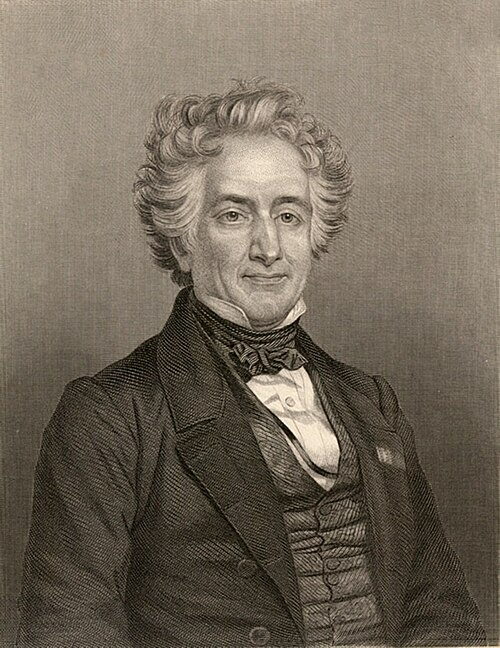
\includegraphics[width=\linewidth]{images/book3/chevreul.jpg}
\end{minipage}\hfill
\begin{minipage}[t]{0.74\linewidth}
\vspace{0pt}
मिशेल यूजीन शेव्रोल ने 1823 में प्रकाशित एक अध्ययन में दिखाया कि वसाएँ ग्लिसरॉल और
वसा अम्लों के यौगिक हैं, जिन्हें उन्होंने पृथक किया और नाम दिए (स्टिऐरिक, ओलेइक, ब्यूटिरिक अम्ल), और यह कि
\omterm{def:b2:acyl-substitution:saponification}{साबुनीकरण} उन्हें इन दो भागों में विभाजित करता है। उनके काम ने साबुन और मोमबत्ती बनाने को
रसायन में बदल दिया; वे 102 वर्ष तक जीवित रहे। (चित्र: निकोला युस्ताश मोरें, सार्वजनिक अधिकार-क्षेत्र, विकिमीडिया
कॉमन्स।)
\end{minipage}
\end{history}

\begin{safety}{\ghs[5mm]{GHS02}\,\ghs[5mm]{GHS05}\,\ghs[5mm]{GHS06}}
थायोनिल क्लोराइड और \omterm{def:b2:acyl-substitution:derivative}{ऐसिल क्लोराइड} जल से प्रचंड अभिक्रिया करते हैं और संक्षारक गैसें मुक्त करते हैं; इन्हें
शुष्क अवस्था में, धूम-हुड में सँभाला जाता है। लिथियम ऐलुमिनियम हाइड्राइड जल के संपर्क में जल उठता है; इसका
आधिक्य अंत में सावधानी से नष्ट किया जाता है। सांद्र सोडियम हाइड्रॉक्साइड त्वचा और आँखों के लिए
संक्षारक है। मेथेनॉल विषैला और ज्वलनशील है।
% ledger: ghs:SOCl2, ghs:ethanoyl-chloride, ghs:LiAlH4, ghs:NaOH, ghs:methanol
\end{safety}

\section{अभ्यास}

\begin{exercise}[$\star$]\label{exo:b2:acyl-substitution:1}
जल के प्रति अभिक्रियाशीलता के क्रम में रखिए: एथिल एथेनोएट, एथेनॉयल क्लोराइड, एथेनैमाइड, एथेनोइक
ऐनहाइड्राइड।
\end{exercise}

\begin{exercise}[$\star$]\label{exo:b2:acyl-substitution:2}
एथेनॉयल क्लोराइड के उत्पाद दीजिए, इनके साथ: जल; एथेनॉल; अमोनिया (2 तुल्यांक);
सोडियम एथेनोएट; ट्राइएथिलऐमीन के साथ डाइमेथिलऐमीन।
\end{exercise}

\begin{exercise}[$\star$]\label{exo:b2:acyl-substitution:3}
सोडियम हाइड्रॉक्साइड द्वारा मेथिल बेन्ज़ोएट का \omterm{def:b2:acyl-substitution:saponification}{साबुनीकरण} लिखिए और एस्टर के \qty{13.6}{g} के लिए आवश्यक सोडियम
हाइड्रॉक्साइड का द्रव्यमान परिकलित कीजिए।
\end{exercise}

\begin{exercise}[$\star$]\label{exo:b2:acyl-substitution:4}
4-हाइड्रॉक्सीब्यूटेनोइक अम्ल से बनने वाला \omterm{def:b2:acyl-substitution:lactone}{लैक्टोन} खींचिए और उसके वलय का आकार बताइए।
\end{exercise}

\begin{exercise}[$\star\star$]\label{exo:b2:acyl-substitution:5}
अमोनिया के साथ एथिल एथेनोएट की अभिक्रिया की क्रियाविधि लिखिए।
\end{exercise}

\begin{exercise}[$\star\star$]\label{exo:b2:acyl-substitution:6}
ऐस्पिरिन सैलिसिलिक अम्ल (2-हाइड्रॉक्सीबेन्ज़ोइक अम्ल) और एथेनोइक ऐनहाइड्राइड से बनाई जाती है। सैलिसिलिक अम्ल का
कौन-सा समूह अभिक्रिया करता है, और उपोत्पाद क्या है?
\end{exercise}

\begin{exercise}[$\star\star$]\label{exo:b2:acyl-substitution:7}
एथिल एथेनोएट को आधिक्य मेथिलमैग्नीशियम ब्रोमाइड से, फिर तनु अम्ल से उपचारित किया जाता है।
उत्पाद दीजिए और समझाइए कि कीटोन को पृथक क्यों नहीं किया जा सकता।
\end{exercise}

\begin{exercise}[$\star\star$]\label{exo:b2:acyl-substitution:8}
अभ्यास 4 के \omterm{def:b2:acyl-substitution:lactone}{लैक्टोन} के \ce{LiAlH4} द्वारा अपचयन का उत्पाद दीजिए।
\end{exercise}

\begin{exercise}[$\star\star$]\label{exo:b2:acyl-substitution:9}
$K = 4$ के साथ एथेनॉल के एक, फिर तीन तुल्यांकों से एस्टरीकृत एथेनोइक अम्ल का अंश परिकलित
कीजिए। कौन-सी अन्य विधि अभिक्रिया को आगे बढ़ाती है?
\end{exercise}

\begin{exercise}[$\star\star\star$]\label{exo:b2:acyl-substitution:10}
बेन्ज़ोइक अम्ल से \textit{N},\textit{N}-डाइएथिलबेन्ज़ैमाइड बनाइए, और समझाइए कि अम्ल को
डाइएथिलऐमीन के साथ मिलाकर हल्का गर्म करने से इसके बजाय एक लवण क्यों मिलता है।
\end{exercise}

\begin{exercise}[$\star\star\star$]\label{exo:b2:acyl-substitution:11}
किसी वसा का \omterm{def:b2:acyl-substitution:saponification}{साबुनीकरण} मान पोटैशियम हाइड्रॉक्साइड का mg में वह द्रव्यमान है जो उसके \qty{1}{g} के
\omterm{def:b2:acyl-substitution:saponification}{साबुनीकरण} के लिए चाहिए। ट्राइओलीन (\qty{885.4}{g/mol}; KOH \qty{56.11}{g/mol}) के लिए इसे परिकलित कीजिए।
\end{exercise}

\begin{exercise}[$\star\star\star$]\label{exo:b2:acyl-substitution:12}
किसी अणु पर एक एस्टर, एक ऐमाइड और एक कीटोन है। \ce{NaBH4} किस समूह (या समूहों) का अपचयन करता है, और
\ce{LiAlH4} किनका? हर स्थिति में आपको क्या प्राप्त होता है?
\end{exercise}

\section{समस्या: तलने के तेल से बायोडीज़ल}

\begin{problem}[{सप्ताहांत समस्या --- ट्राइओलीन और उसका मोलर द्रव्यमान, मेथेनॉल के साथ उसका
पार-एस्टरीकरण और क्षारक की भूमिका, मुक्त अम्लों और जल के साथ पार्श्व अभिक्रिया, और प्रति
टन तेल लब्धियाँ}]
\label{pb:b2:acyl-substitution:1}
तेल को शुद्ध ट्राइओलीन मानिए, जो ओलेइक अम्ल (\ce{C17H33COOH}) का ट्राइग्लिसराइड है। मोलर द्रव्यमान
(\unit{g/mol}): C 12.011, H 1.008, O 15.999, Na 22.990। ग्लिसरॉल प्रोपेन-1,2,3-ट्राइऑल है।
% ledger: aw:C, aw:H, aw:O, aw:Na, ghs:methanol, ghs:NaOH

\medskip
\noindent\textbf{भाग I --- ट्राइओलीन।}
\begin{enumerate}
  \item ओलेइक अम्ल और ग्लिसरॉल के सूत्र दीजिए।
  \item ट्राइओलीन का सूत्र लिखिए और उसका मोलर द्रव्यमान परिकलित कीजिए।
  \item इसमें कितने एस्टर समूह हैं?
  \item ओलेइक अम्ल में एक cis द्वि-आबंध है। इससे समृद्ध तेल कमरे के ताप पर द्रव क्यों होते हैं?
  \item ट्राइओलीन का \omterm{def:b2:acyl-substitution:saponification}{साबुनीकरण} क्या देगा?
  \item रासायनिक रूप से बायोडीज़ल क्या है?
\end{enumerate}

\medskip
\noindent\textbf{भाग II --- \omterm{def:b2:acyl-substitution:transesterification}{पार-एस्टरीकरण}।}
\begin{enumerate}[resume]
  \item मेथेनॉल के साथ ट्राइओलीन का \omterm{def:b2:acyl-substitution:transesterification}{पार-एस्टरीकरण} लिखिए।
  \item उत्प्रेरक के रूप में क्षारक (सोडियम मेथॉक्साइड या हाइड्रॉक्साइड) क्यों प्रयुक्त होता है?
  \item पहले आदान-प्रदान का \omterm{def:b2:acyl-substitution:nas}{चतुष्फलकीय मध्यवर्ती} खींचिए।
  \item मेथेनॉल आधिक्य में (तीन के बजाय छह तुल्यांक) क्यों प्रयुक्त होता है?
  \item ग्लिसरॉल मेथिल एस्टरों के साथ मिश्रणीय नहीं है। इससे कैसे सहायता मिलती है?
  \item क्या आदर्श अभिक्रिया में उत्प्रेरक उपभुक्त होता है?
\end{enumerate}

\medskip
\noindent\textbf{भाग III --- मुक्त अम्ल और जल।}
\begin{enumerate}[resume]
  \item प्रयुक्त तलने के तेल में मुक्त ओलेइक अम्ल होता है। यह क्षारक के साथ क्या करता है?
  \item क्षारक की उपस्थिति में जल मेथिल एस्टरों के साथ क्या करता है?
  \item बना साबुन बाधा क्यों है?
  \item मुक्त अम्लों को पहले, बिना क्षारक के, कैसे हटाया जा सकता है?
  \item अभिक्रिया से पहले तेल को सुखाना क्यों आवश्यक है?
\end{enumerate}

\medskip
\noindent\textbf{भाग IV --- प्रति टन तेल।}
\begin{enumerate}[resume]
  \item एक टन में ट्राइओलीन की मात्रा परिकलित कीजिए।
  \item उपभुक्त मेथेनॉल का द्रव्यमान परिकलित कीजिए।
  \item बने मेथिल ओलिएट का द्रव्यमान परिकलित कीजिए।
  \item द्रव्यमान संरक्षण की जाँच कीजिए।
  \item द्रव्यमान से 2~\% मुक्त ओलेइक अम्ल वाले तेल को सोडियम हाइड्रॉक्साइड से उपचारित किया जाता है: प्रति टन अम्ल द्वारा
        उपभुक्त सोडियम हाइड्रॉक्साइड का द्रव्यमान परिकलित कीजिए।
  \item प्रति टन ट्राइओलीन सह-उत्पादित ग्लिसरॉल का द्रव्यमान परिकलित कीजिए।
\end{enumerate}
\end{problem}
